%!TEX root = ../../../../build/bioseqdb_thesis/_prebuild/main.tex
% type: thesis
% title:
%   pl: Zintegrowane i praktyczne rozwiązanie bazodanowe do przechowywania i wydajnego przetwarzania dużych zbiorów danych genomicznych
%   en: An integrated and practical database solution for storage and efficient processing of large genomic datasets
% major: Computer Science
% subject: !socrateserasmus 11.3
% classification:
%   - Applied computing
%   - Life and medical sciences
%   - Bioinformatics
% keywords:
%   - sequence alignment
%   - bioinformatics
%   - minimap2
%   - PostgreSQL
%   - databases
%   - genomic data management
%   - SIMD
%   - GPU computing
% author:
%   name: Piotr Styczyński
%   id: 386038
% created: 2026-07-28
% languages:
%   - en-US
% chapters:
%   - !partial
%     title: Biological foundations of sequence analysis
%     path: chapters/01_biology
%     description: introduces biological sequences and sequencing data. It explains variation and the computational questions that motivate database-resident sequence analysis.
%   - !partial
%     title: Sequence alignment and search strategies
%     path: chapters/02_alignment_foundations
%     description: develops exact dynamic programming and seed-and-extend mapping. It also presents graph-based approaches and the limits of existing tools.
%   - !partial
%     title: Minimizer extraction
%     path: chapters/05_minimizers
%     description: explains minimizer sketching and rolling hashing. It compares the SIMD and Vulkan implementations with minimap2 and SIMD-Minimizers.
%   - !partial
%     title: Chaining seed anchors
%     path: chapters/06_chaining
%     description: derives the chaining objective and compares its scalar RMQ SIMD and GPU forms. It then states the selection policy.
%   - !partial
%     title: Final alignment and postprocessing
%     path: chapters/07_final_alignment_postprocessing_and_preprocessing
%     description: compares KSW2 and Block Aligner, explains SneakySnake filtering and distinguishes the reported alignment statistics.
%   - !partial
%     title: Sequence representations and lazy evaluation
%     path: chapters/09_sequence_abstractions
%     description: develops compact sequence ranges and bit-level views. It then presents fragmented and lazy sequences with PostgreSQL-backed adapters and alphabet dispatch.
%   - !partial
%     title: PostgreSQL API and custom scans
%     path: chapters/10_postgres_custom_scan
%     description: follows an mmsearch expression through planning and batched execution. It explains joins and per-row result substitution.
%   - !partial
%     title: Physical sequence storage in PostgreSQL
%     path: chapters/11_postgres_storage
%     description: explains the columnar-derived storage layout and fragment metadata. It also covers caching and request coordination.
%   - !partial
%     title: Persistent sequence indexes
%     path: chapters/12_index_storage
%     description: describes index construction and storage with compatibility checks and selective cold loading. It also explains updates and differences from minimap2 indexes.
%%   - !partial
%%     title: BioSeqDB architecture
%%     path: chapters/13_bioseqdb_architecture
%%     description: connects algorithm selection and oneTBB scheduling to a reusable processing core. It also covers sequence ingestion, remote access, code generation, validation and authorship.
%   - !partial
%     title: Benchmarking and performance evaluation
%     path: chapters/16_benchmarking
%     description: measuring overall performance of BioseqDB
%   - !partial
%     title: Conclusions
%     path: chapters/17_conclusion
%     description: answers the research questions and summarizes the final system. It identifies the principal limitations and possible extensions.
% authorship: !partial
%   title: Authorship, development and AI assistance
%   path: chapters/18_authorship
% appendices:
%   - !partial
%     title: A runnable SQL walkthrough
%     path: appendices/02_sql_walkthrough
%   - !partial
%     title: Configuration reference
%     path: appendices/03_configuration_reference
% xrenderonly: chapters/05_minimizers

% Keep thesis hyperlinks legible on a white page.  `breaklinks` also permits
% linked bibliography fields (for example, long conference titles) to wrap.
\hypersetup{
  breaklinks=true,
  linkcolor=blue,
  citecolor=blue,
  urlcolor=blue
}

\if\dataeq{renderonly}{??}

% Keep the generated metadata while giving the visible front matter proper
% punctuation and a classification block that cannot strand its final item on
% the following page.
\keywords{sequence alignment, bioinformatics, minimap2, PostgreSQL, databases,
    genomic data management, SIMD, GPU computing}
\dziedzina{11.3 Informatics and Computer Science}
\klasyfikacja{\mbox{Applied computing, life and medical sciences, bioinformatics}}

\begin{abstract}
    % This abstract is too long for the class's vertically centered layout.
    % Cancel its opening stretch so the complete front matter uses the page.
    \vfilneg
    % Keep the Polish-title label and its two-line value on this title page.
    \enlargethispage{4\baselineskip}
The field of bioinformatics and genomic data analysis is growing rapidly, however, many tools for fundamental tasks such as alignment calculation and clustering remain 
either outdated or difficult to use. Finding a user-friendly system that supports essential bioinformatics workflows is still a major challenge. 
Current solutions are often outdated, hard to use, and lack integration capabilities that would allow them to work seamlessly 
with other tools in the research ecosystem. 
The most popular tool remains the Blast+ toolkit maintained by the National Library of Medicine.
 At the same time, there is a large number of open-source aligners available, such as minimap, mmseqs, bwa, and Kraken. 
 Many of these tools suffer from significant technical debt, use incompatible data formats, and are generally difficult to deploy and operate at scale.

I created BioseqDB to address this shortcominds. BisoeqDB is Postgres extension that provides performant columnar storage with compression for storing very large sequences of any sizes, without the need to preprocess the data.
BioseqDB offers efficient scalar CPU algorithms and optimised SIMD algorithms as well as experimental portable Vulkan kernels for GPU.

BioseqDB enable research labs to upload FASTA/FASTQ files directly into the database and perform alignments that in the worst cases can offer up to 120x speedup when RAM is very limited.
In average case for very long sequences, the speedup was up to 10x for indexed queries.

In the implemetation I provide multi-platform implementations that can execute on almost any architectures and custom optimisations which benchmarked comparisons.
\end{abstract}

\makeatletter
% The class defaults are sized for single-digit chapter numbers.  Reserve
% enough width for entries such as 10.10 and 10.10.1 before their titles.
\renewcommand*\l@section{\@dottedtocline{1}{1.5em}{3.0em}}
\renewcommand*\l@subsection{\@dottedtocline{2}{3.8em}{4.0em}}
\renewcommand*\l@subsubsection{\@dottedtocline{3}{7.0em}{5.0em}}
\makeatother
\tableofcontents

\chapter*{Introduction}
    \addcontentsline{toc}{chapter}{Introduction}

    The thesis is structured in the way that each stage of pipeline prosecessing is discussed in chronological order, while the Postgres storage details are addressed later.
    At the end of the thesis I provide samples of usage to demonstrate all the features and unprocessed benchmark results for different scenarios and machines.

    % Keep the chapter roadmap together before the development timeline.
    \begin{itemize}
        \setlength{\itemsep}{0pt}
        \setlength{\parsep}{0pt}
        \foreachdata{chapters}{\chapteri} {
            \chapterbrief{r:\data{chapters.\chapteri.ref}}{\data{chapters.\chapteri.description}}
        }
    \end{itemize}

    This thesis required several years of exploration and experiments.
    I began without a formal background in computational biology, thus
    learning the field was part of the research. I proposed the database
    idea and prepared the initial design, when I was still working for my funded startup.
    I directed the 2022 prototype, whose implementation was written by colleagues and plugged BWA-MEM call directly into Postgres via C bindings.\footnote{\fontsize{7.5}{9}\selectfont 
    The current BioSeqDB is a separate project, designed and written by me.
    It contains no code or intellectual property from the early BWA-MEM integration experiments.}
    The early prototype was to simplistic as technically I still didn't understand how aligners work internally.

    The idea of writing my own alignment software was my long standing dream. I explored the field hobbistically and this thesis stands as the final result of all that work. 

    \begin{center}
    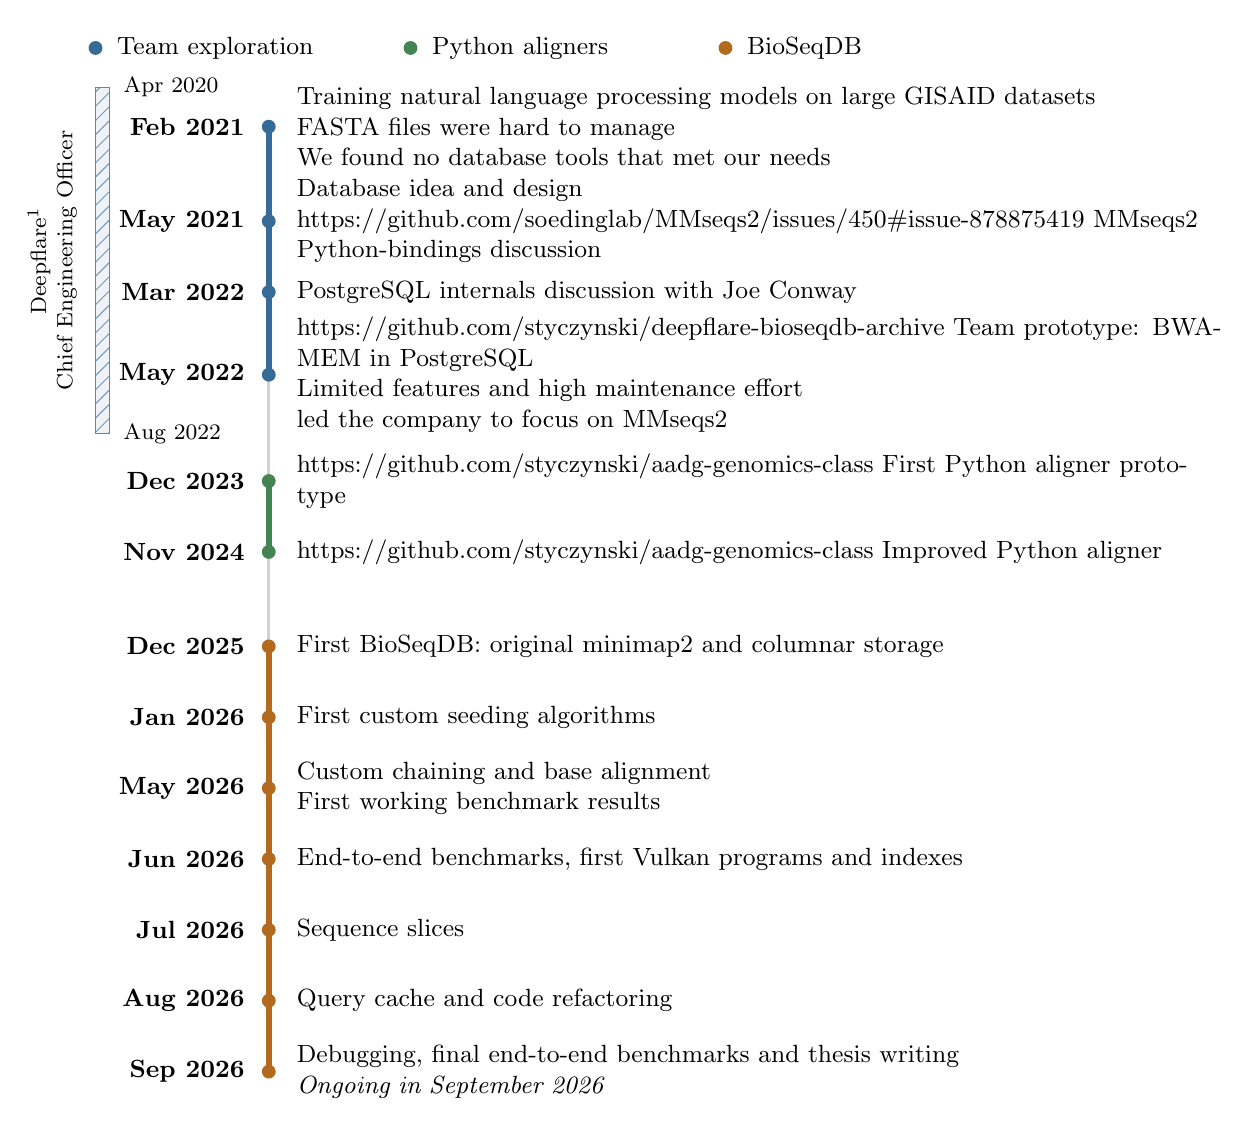
\begin{tikzpicture}[x=1cm,y=1cm,font=\small,
      timeline date/.style={anchor=east,font=\small\bfseries,
        inner sep=0pt},
      timeline event/.style={anchor=west,align=left,text width=11.8cm,
        inner sep=0pt},
      timeline dot/.style={circle,inner sep=0pt,minimum size=5pt}]
      \definecolor{timelineConcept}{HTML}{366B98}
      \definecolor{timelinePython}{HTML}{438452}
      \definecolor{timelineBioseq}{HTML}{B36A1F}

      % A separate striped bar marks the career period beside the milestones.
      \fill[timelineConcept!8] (0,-0.4) rectangle (0.18,-4.8);
      \begin{scope}
        \clip (0,-0.4) rectangle (0.18,-4.8);
        \foreach \timelineStripe in {-5,-4.82,...,-0.2} {
          \draw[timelineConcept!70,line width=0.35pt]
            (-0.04,\timelineStripe) -- (0.22,{\timelineStripe+0.26});
        }
      \end{scope}
      \draw[timelineConcept!80,line width=0.4pt]
        (0,-0.4) rectangle (0.18,-4.8);
      \node[anchor=west,font=\footnotesize,inner sep=0pt]
        at (0.35,-0.4) {Apr 2020};
      \node[anchor=west,font=\footnotesize,inner sep=0pt]
        at (0.35,-4.8) {Aug 2022};
      \node[rotate=90,align=center,font=\footnotesize,inner sep=0pt]
        at (-0.55,-2.6)
        {Deepflare\footnotemark\\Chief Engineering Officer};

      % A compact key names the phases without long explanations.
      \fill[timelineConcept] (0,0.1) circle (2.5pt);
      \node[anchor=west] at (0.15,0.1) {Team exploration};
      \fill[timelinePython] (4,0.1) circle (2.5pt);
      \node[anchor=west] at (4.15,0.1) {Python aligners};
      \fill[timelineBioseq] (8,0.1) circle (2.5pt);
      \node[anchor=west] at (8.15,0.1) {BioSeqDB};

      \draw[black!18,line width=1pt] (2.2,-0.9) -- (2.2,-12.9);
      \draw[timelineConcept,line width=2pt] (2.2,-0.9) -- (2.2,-4.05);
      \draw[timelinePython,line width=2pt] (2.2,-5.4) -- (2.2,-6.3);
      \draw[timelineBioseq,line width=2pt] (2.2,-7.5) -- (2.2,-12.9);

      \foreach \timelineY/\timelineDate/\timelineColor in {
        -0.9/Feb 2021/timelineConcept,
        -2.1/May 2021/timelineConcept,
        -3.0/Mar 2022/timelineConcept,
        -4.05/May 2022/timelineConcept,
        -5.4/Dec 2023/timelinePython,
        -6.3/Nov 2024/timelinePython,
        -7.5/Dec 2025/timelineBioseq,
        -8.4/Jan 2026/timelineBioseq,
        -9.3/May 2026/timelineBioseq,
        -10.2/Jun 2026/timelineBioseq,
        -11.1/Jul 2026/timelineBioseq,
        -12.0/Aug 2026/timelineBioseq,
        -12.9/Sep 2026/timelineBioseq} {
        \node[timeline date] at (1.9,\timelineY) {\timelineDate};
        \node[timeline dot,fill=\timelineColor] at (2.2,\timelineY) {};
      }

      \node[timeline event] at (2.55,-0.9)
        {Training natural language processing models on large GISAID datasets\\
         FASTA files were hard to manage\\
         We found no database tools that met our needs};
      \node[timeline event] at (2.55,-2.1)
        {Database idea and design\\
         \href{https://github.com/soedinglab/MMseqs2/issues/450\#issue-878875419}
           {MMseqs2 Python-bindings discussion}};
      \node[timeline event] at (2.55,-3.0)
        {PostgreSQL internals discussion with Joe Conway};
      \node[timeline event] at (2.55,-4.05)
        {\href{https://github.com/styczynski/deepflare-bioseqdb-archive}
           {Team prototype: BWA-MEM in PostgreSQL}\\
         Limited features and high maintenance effort\\
         led the company to focus on MMseqs2};
      \node[timeline event] at (2.55,-5.4)
        {\href{https://github.com/styczynski/aadg-genomics-class}
           {First Python aligner prototype}};
      \node[timeline event] at (2.55,-6.3)
        {\href{https://github.com/styczynski/aadg-genomics-class}
           {Improved Python aligner}};
      \node[timeline event] at (2.55,-7.5)
        {First BioSeqDB: original minimap2 and columnar storage};
      \node[timeline event] at (2.55,-8.4)
        {First custom seeding algorithms};
      \node[timeline event] at (2.55,-9.3)
        {Custom chaining and base alignment\\First working benchmark results};
      \node[timeline event] at (2.55,-10.2)
        {End-to-end benchmarks, first Vulkan programs and indexes};
      \node[timeline event] at (2.55,-11.1)
        {Sequence slices};
      \node[timeline event] at (2.55,-12.0)
        {Query cache and code refactoring};
      \node[timeline event] at (2.55,-12.9)
        {Debugging, final end-to-end benchmarks and thesis writing\\
         \textit{Ongoing in September 2026}};
    \end{tikzpicture}
    \label{sec:introduction-timeline}
    \end{center}
    {\small\noindent Project history\par}
    \footnotetext{\fontsize{7.5}{9}\selectfont I was a co-founder (shareholder) until 15 July 2022 (KRS update on 3 Jun 2022) in Covid Genomics Sp. z o.o. (registered in Poland in Jun 2020, KRS 0000846289) which then changed its legal name to CGen Sp. z o.o. (on 3 Jun 2022) and then changed its branding name to Deepflare (on Jul 2022). I was also a Chief Engineering Officer from 1 Apr 2020 till 31 Aug 2022.}

\foreachdata{chapters}{\chapteri} {
    \defchapter{\data{chapters.\chapteri.title}}{r:\data{chapters.\chapteri.ref}}
    \datapartial{chapters.\chapteri}
}

\chapter*{Authorship, development and AI assistance}
\addcontentsline{toc}{chapter}{Authorship, development and AI assistance}
\datapartial{authorship}

\else
\foreachdata{chapters}{\chapteri} {
    \ddef\renderedchr{renderonly}
    \if\dataeq{chapters.\chapteri.ref}\renderedchr
        \datapartial{chapters.\chapteri}
    \fi
}
\fi

\if\dataeq{hasbibliography}{true}
  \begingroup
    \sloppy
    \raggedright
    \setlength{\emergencystretch}{3em}
    \printbibliography[heading=bibintoc,title={References}]
  \endgroup
\fi

% Appendices follow the references and do not enter the chapter synopsis.
\if\dataeq{renderonly}{??}
  \appendix
  \renewcommand{\thechapter}{\arabic{chapter}}
  \renewcommand{\theHchapter}{appendix.\arabic{chapter}}
  \addtocontents{toc}{\protect\setcounter{tocdepth}{1}}
  \foreachdata{appendices}{\appendixi} {
    \chapter{\data{appendices.\appendixi.title}}
    \label{r:\data{appendices.\appendixi.ref}}
    \datapartial{appendices.\appendixi}
  }
\fi
